% questions.tex —— 2016 年·全国Ⅰ卷·文科 · 题目内容片段（无答案）
% 由 tools/generate_projects.py 依来源总账自 2016/2016_数学真题_全国1文_试题.md 生成，勿手改（改源 MD 后重跑）


\gkpart{数学}

\begin{gktip}
\textbf{来源说明}：本题面依据固定源 PDF 两页 A3 页面逐题核对，原卷印刷页码 1001–1002。固定源不附答案；本文件仅为题面规范源。
\end{gktip}

\gkpart{一、选择题}

\begin{question}
\gkti{1}设集合 \(A=\{1,3,5,7\}\)，\(B=\{x\mid 2\leq x\leq 5\}\)，则 \(A\cap B=\)（　）

\begin{gkopts}(2)
\task （A）\(\{1,3\}\)
\task （B）\(\{3,5\}\)
\task （C）\(\{5,7\}\)
\task （D）\(\{1,7\}\)
\end{gkopts}

\end{question}
\begin{question}
\gkti{2}设 \((1+2i)(a+i)\) 的实部与虚部相等，其中 \(a\) 为实数，则 \(a=\)（　）

\begin{gkopts}(2)
\task （A）\(-3\)
\task （B）\(-2\)
\task （C）\(2\)
\task （D）\(3\)
\end{gkopts}

\end{question}
\begin{question}
\gkti{3}为美化环境，从红、黄、白、紫 4 种颜色的花中任选 2 种花种在一个花坛中，余下的 2 种花种在另一个花坛中，则红色和紫色的花不在同一花坛的概率是（　）

\begin{gkopts}(2)
\task （A）\(\dfrac{1}{3}\)
\task （B）\(\dfrac{1}{2}\)
\task （C）\(\dfrac{2}{3}\)
\task （D）\(\dfrac{5}{6}\)
\end{gkopts}

\end{question}
\begin{question}
\gkti{4}\(\triangle ABC\) 的内角 \(A,B,C\) 的对边分别为 \(a,b,c\)。已知 \(a=\sqrt{5}\)，\(c=2\)，\(\cos A=\dfrac{2}{3}\)，则 \(b=\)（　）

\begin{gkopts}(2)
\task （A）\(\sqrt{2}\)
\task （B）\(\sqrt{3}\)
\task （C）\(2\)
\task （D）\(3\)
\end{gkopts}

\end{question}
\begin{question}
\gkti{5}直线 \(l\) 经过椭圆的一个顶点和一个焦点，若椭圆中心到 \(l\) 的距离为其短轴长的 \(\dfrac{1}{4}\)，则该椭圆的离心率为（　）

\begin{gkopts}(2)
\task （A）\(\dfrac{1}{3}\)
\task （B）\(\dfrac{1}{2}\)
\task （C）\(\dfrac{2}{3}\)
\task （D）\(\dfrac{3}{4}\)
\end{gkopts}

\end{question}
\begin{question}
\gkti{6}将函数 \(y=2\sin\left(2x+\dfrac{\pi}{6}\right)\) 的图象向右平移 \(\dfrac{1}{4}\) 个周期后，所得图象对应的函数为（　）

   （A）\(y=2\sin\left(2x+\dfrac{\pi}{4}\right)\)　（B）\(y=2\sin\left(2x+\dfrac{\pi}{3}\right)\)

   （C）\(y=2\sin\left(2x-\dfrac{\pi}{4}\right)\)　（D）\(y=2\sin\left(2x-\dfrac{\pi}{3}\right)\)

\Needspace{0.4\textheight}
\end{question}
\begin{question}
\gkti{7}如图，某几何体的三视图是三个半径相等的圆及每个圆中两条相互垂直的半径。若该几何体的体积是 \(\dfrac{28\pi}{3}\)，则它的表面积是（　）
\nopagebreak[4]
\begin{center}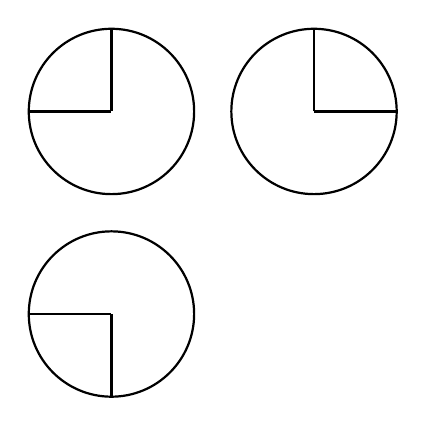
\begin{tikzpicture}[scale=1.05]
\draw[thick] (0,0) circle (1);
\draw[thick] (0,0) -- (0,1) (-1,0) -- (0,0);

\draw[thick] (2.45,0) circle (1);
\draw[thick] (2.45,0) -- (2.45,1) (2.45,0) -- (3.45,0);

\draw[thick] (0,-2.45) circle (1);
\draw[thick] (0,-2.45) -- (-1,-2.45) (0,-2.45) -- (0,-3.45);
\end{tikzpicture}
\end{center}
\nopagebreak[4]
\begin{gkopts}(2)
\task （A）\(17\pi\)
\task （B）\(18\pi\)
\task （C）\(20\pi\)
\task （D）\(28\pi\)
\end{gkopts}

\end{question}
\begin{question}
\gkti{8}若 \(a>b>0\)，\(0<c<1\)，则（　）

   （A）\(\log_a c<\log_b c\)　（B）\(\log_c a<\log_c b\)

   （C）\(a^c<b^c\)　（D）\(c^a>c^b\)

\Needspace{0.4\textheight}
\end{question}
\begin{question}
\gkti{9}函数 \(y=2x^2-e^{|x|}\) 在 \([-2,2]\) 的图象大致为（　）
\nopagebreak[4]
\begin{center}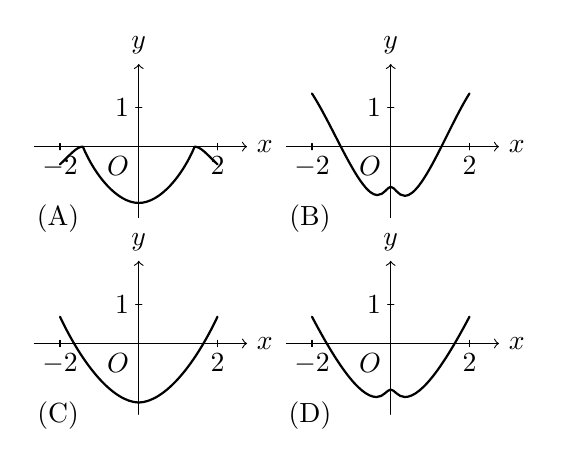
\begin{tikzpicture}[x=0.5cm,y=0.5cm,line cap=round,line join=round]
\begin{scope}
  \draw[->] (-2.65,0) -- (2.75,0) node[right] {$x$};
  \draw[->] (0,-1.8) -- (0,2.1) node[above] {$y$};
  \draw (-2,0.08) -- (-2,-0.08) (2,0.08) -- (2,-0.08);
  \draw (0.08,1) -- (-0.08,1);
  \node[below] at (-2,0) {$-2$};
  \node[below] at (2,0) {$2$};
  \node[left] at (0,1) {$1$};
  \node[below left] at (0,0) {$O$};
  \draw[thick] (-2,-0.45)
    .. controls (-1.72,-0.18) and (-1.57,0) .. (-1.42,0)
    .. controls (-1.12,-0.72) and (-0.55,-1.43) .. (0,-1.43)
    .. controls (0.55,-1.43) and (1.12,-0.72) .. (1.42,0)
    .. controls (1.57,0) and (1.72,-0.18) .. (2,-0.45);
  \node at (-2.05,-1.83) {(A)};
\end{scope}

\begin{scope}[shift={(6.4,0)}]
  \draw[->] (-2.65,0) -- (2.75,0) node[right] {$x$};
  \draw[->] (0,-1.8) -- (0,2.1) node[above] {$y$};
  \draw (-2,0.08) -- (-2,-0.08) (2,0.08) -- (2,-0.08);
  \draw (0.08,1) -- (-0.08,1);
  \node[below] at (-2,0) {$-2$};
  \node[below] at (2,0) {$2$};
  \node[left] at (0,1) {$1$};
  \node[below left] at (0,0) {$O$};
  \draw[thick] (-2,1.35)
    .. controls (-1.43,0.47) and (-0.79,-1.23) .. (-0.34,-1.23)
    .. controls (-0.17,-1.23) and (-0.08,-1.02) .. (0,-1.02)
    .. controls (0.10,-1.02) and (0.18,-1.25) .. (0.36,-1.25)
    .. controls (0.82,-1.25) and (1.45,0.48) .. (2,1.35);
  \node at (-2.05,-1.83) {(B)};
\end{scope}

\begin{scope}[shift={(0,-5)}]
  \draw[->] (-2.65,0) -- (2.75,0) node[right] {$x$};
  \draw[->] (0,-1.8) -- (0,2.1) node[above] {$y$};
  \draw (-2,0.08) -- (-2,-0.08) (2,0.08) -- (2,-0.08);
  \draw (0.08,1) -- (-0.08,1);
  \node[below] at (-2,0) {$-2$};
  \node[below] at (2,0) {$2$};
  \node[left] at (0,1) {$1$};
  \node[below left] at (0,0) {$O$};
  \draw[thick] (-2,0.68)
    .. controls (-1.42,-0.55) and (-0.66,-1.48) .. (0,-1.5)
    .. controls (0.66,-1.48) and (1.42,-0.55) .. (2,0.68);
  \node at (-2.05,-1.83) {(C)};
\end{scope}

\begin{scope}[shift={(6.4,-5)}]
  \draw[->] (-2.65,0) -- (2.75,0) node[right] {$x$};
  \draw[->] (0,-1.8) -- (0,2.1) node[above] {$y$};
  \draw (-2,0.08) -- (-2,-0.08) (2,0.08) -- (2,-0.08);
  \draw (0.08,1) -- (-0.08,1);
  \node[below] at (-2,0) {$-2$};
  \node[below] at (2,0) {$2$};
  \node[left] at (0,1) {$1$};
  \node[below left] at (0,0) {$O$};
  \draw[thick] (-2,0.68)
    .. controls (-1.43,-0.40) and (-0.82,-1.36) .. (-0.36,-1.36)
    .. controls (-0.18,-1.36) and (-0.09,-1.17) .. (0,-1.17)
    .. controls (0.09,-1.17) and (0.18,-1.36) .. (0.36,-1.36)
    .. controls (0.82,-1.36) and (1.43,-0.40) .. (2,0.68);
  \node at (-2.05,-1.83) {(D)};
\end{scope}
\end{tikzpicture}
\end{center}
\nopagebreak[4]
\Needspace{0.4\textheight}
\end{question}
\begin{question}
\gkti{10}执行下面的程序图，如果输入的 \(x=0,y=1,n=1\)，则输出 \(x,y\) 的值满足（　）
\nopagebreak[4]
\begin{center}\begin{tikzpicture}[line cap=round,line join=round]
% 开始与输入
\draw[rounded corners=3pt] (-0.65,6.3) rectangle (0.65,6.9);
\node at (0,6.6) {开始};
\draw (-1.55,5.3) -- (1.25,5.3) -- (1.55,4.65) -- (-1.25,4.65) -- cycle;
\node at (0,4.98) {输入 $x,y,n$};
\draw[->] (0,6.3) -- (0,5.3);

% 更新与循环判断
\draw (-2.75,3.15) rectangle (2.75,4.25);
\node at (0,3.85) {$x=x+\dfrac{n-1}{2},\quad y=ny$};
\draw (0,4.65) -- (0,4.48);
\draw[->] (0,4.48) -- (0,4.25);

\draw (0,1.95) -- (2.15,1.45) -- (0,0.95) -- (-2.15,1.45) -- cycle;
\node at (0,1.45) {$x^2+y^2\geq 36$};
\draw[->] (0,3.15) -- (0,1.95);

% 否分支先递增 n，再返回更新框
\draw (-4.9,2.3) rectangle (-2.7,2.8);
\node at (-3.8,2.55) {$n=n+1$};
\draw (-2.15,1.45) -- (-3.8,1.45);
\draw[->] (-3.8,1.45) -- (-3.8,2.3);
\draw[->] (-3.8,2.8) -- (-3.8,4.48);
\draw[->] (-3.8,4.48) -- (0,4.48);
\node at (-2.65,1.2) {否};

% 是分支输出并结束
\draw (-1.3,0.25) -- (1.3,0.25) -- (1.05,-0.45) -- (-1.55,-0.45) -- cycle;
\draw[->] (0,0.95) -- (0,0.25);
\node at (-0.38,0.68) {是};
\node at (-0.25,-0.1) {输出 $x,y$};
\draw[->] (0,-0.45) -- (0,-0.85);
\draw[rounded corners=3pt] (-0.65,-1.45) rectangle (0.65,-0.85);
\node at (0,-1.15) {结束};
\end{tikzpicture}
\end{center}
\nopagebreak[4]
\begin{gkopts}(2)
\task （A）\(y=2x\)
\task （B）\(y=3x\)
\task （C）\(y=4x\)
\task （D）\(y=5x\)
\end{gkopts}

\end{question}
\begin{question}
\gkti{11}平面 \(\alpha\) 过正方体 \(ABCD-A_1B_1C_1D_1\) 的顶点 \(A\)，\(\alpha\parallel\) 平面 \(CB_1D_1\)，\(\alpha\cap\) 平面 \(ABCD=m\)，\(\alpha\cap\) 平面 \(ABB_1A_1=n\)，则 \(m,n\) 所成角的正弦值为（　）

\begin{gkopts}(2)
\task （A）\(\dfrac{\sqrt{3}}{2}\)
\task （B）\(\dfrac{\sqrt{2}}{2}\)
\task （C）\(\dfrac{\sqrt{3}}{3}\)
\task （D）\(\dfrac{1}{3}\)
\end{gkopts}

\end{question}
\begin{question}
\gkti{12}若函数 \(f(x)=x-\dfrac{1}{3}\sin 2x+a\sin x\) 在 \(( -\infty,+\infty )\) 单调递增，则 \(a\) 的取值范围是（　）

\begin{gkopts}(1)
\task （A）\([-1,1]\)
\task （B）\([-1,\dfrac{1}{3}]\)
\task （C）\([-\dfrac{1}{3},\dfrac{1}{3}]\)
\task （D）\([-1,-\dfrac{1}{3}]\)
\end{gkopts}

\end{question}
\gkpart{二、填空题}

\begin{question}
\gkti{13}设向量 \(\boldsymbol{a}=(x,x+1)\)，\(\boldsymbol{b}=(1,2)\)，且 \(\boldsymbol{a}\perp\boldsymbol{b}\)，则 \(x=\)\gkblank{}。

\end{question}
\begin{question}
\gkti{14}已知 \(\theta\) 是第四象限角，且 \(\sin\left(\theta+\dfrac{\pi}{4}\right)=\dfrac{3}{5}\)，则 \(\tan\left(\theta-\dfrac{\pi}{4}\right)=\)\gkblank{}。

\end{question}
\begin{question}
\gkti{15}设直线 \(y=x+2a\) 与圆 \(C:x^2+y^2-2ay-2=0\) 相交于 \(A,B\) 两点，若 \(|AB|=2\sqrt{3}\)，则圆 \(C\) 的面积为\gkblank{}。

\end{question}
\begin{question}
\gkti{16}某高科技企业生产产品 \(A\) 和产品 \(B\)，需要甲、乙两种新型材料。生产一件产品 \(A\) 需要甲材料 \(1.5\ \mathrm{kg}\)、乙材料 \(1\ \mathrm{kg}\)，用 5 个工时；生产一件产品 \(B\) 需要甲材料 \(0.5\ \mathrm{kg}\)、乙材料 \(0.3\ \mathrm{kg}\)，用 3 个工时；生产一件产品 \(A\) 的利润为 2100 元，生产一件产品 \(B\) 的利润为 900 元。该企业现有甲材料 150 kg、乙材料 90 kg，则在不超过 600 个工时的条件下，生产产品 \(A\)、产品 \(B\) 的利润之和的最大值为\gkblank{}元。

\end{question}
\gkpart{三、解答题}

\begin{question}
\gkti{17}已知 \(\{a_n\}\) 是公差为 3 的等差数列，数列 \(\{b_n\}\) 满足 \(b_1=1\)，\(b_2=\dfrac{1}{3}\)，\(a_nb_{n+1}+b_{n+1}=nb_n\)。

   （1）　求 \(\{a_n\}\) 的通项公式；

   （2）　求 \(\{b_n\}\) 的前 \(n\) 项和。

\Needspace{0.4\textheight}
\end{question}
\begin{question}
\gkti{18}如图，在已知正三棱锥 \(P-ABC\) 的侧面是直角三角形，\(PA=6\)，顶点 \(P\) 在平面 \(ABC\) 内的正投影为点 \(D\)，\(D\) 在平面 \(PAB\) 内的正投影为点 \(E\)，连接 \(PE\) 并延长交 \(AB\) 于点 \(G\)。
\nopagebreak[4]
\begin{center}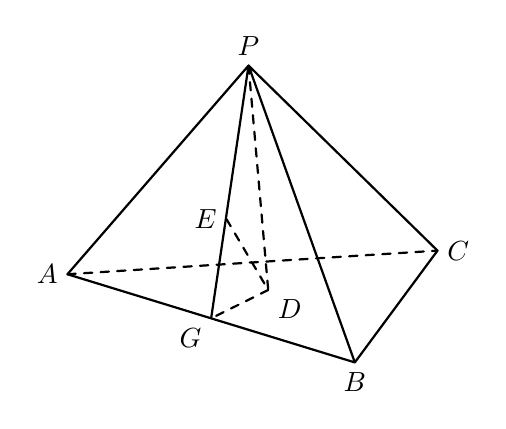
\begin{tikzpicture}[line cap=round,line join=round]
\coordinate (A) at (0,0);
\coordinate (B) at (3.65,-1.12);
\coordinate (C) at (4.7,0.3);
\coordinate (P) at (2.3,2.65);
\coordinate (G) at (1.825,-0.56);
\coordinate (E) at (2.02,0.70);
\coordinate (D) at (2.55,-0.20);

% 隐线与内部构造
\draw[thick,dashed] (A)--(C) (P)--(D) (E)--(D) (D)--(G);
% 棱与 PE 延长线 PG
\draw[thick] (A)--(B)--(C) (A)--(P) (B)--(P) (C)--(P) (P)--(G);

\node[left] at (A) {$A$};
\node[below] at (B) {$B$};
\node[right] at (C) {$C$};
\node[above] at (P) {$P$};
\node[left] at (E) {$E$};
\node[below right] at (D) {$D$};
\node[below left] at (G) {$G$};
\end{tikzpicture}
\end{center}
\nopagebreak[4]
   （1）　证明 \(G\) 是 \(AB\) 的中点；

   （2）　如图，在图中作出点 \(E\) 在平面 \(PAC\) 内的正投影 \(F\)（说明做法及理由），并求四面体 \(PDEF\) 的体积。

\Needspace{0.4\textheight}
\end{question}
\begin{question}
\gkti{19}某公司计划购买 1 台机器，该种机器使用三年后即被淘汰，机器有一易损零件。在购进机器时，可以额外购买这种零件作为备件，每个 200 元。在机器使用期间，如果备件不足再购买，则每个 500 元。现需决策在购买机器时应同时购买几个易损零件，为此搜集并整理了 100 台这种机器在三年试用期内更换的易损零件数，得下面柱状图：
\nopagebreak[4]
\begin{center}\begin{tikzpicture}[x=0.92cm,y=0.15cm,line cap=butt,line join=round]
% 频数轴与横轴
\draw[->,thick] (0,0) -- (0,27.2);
\draw[->,thick] (0,0) -- (7.05,0);
\node[above right] at (0,26.1) {频数};
\node[below left] at (0,0) {$0$};

% 频数参考虚线，延伸到对应柱的左边缘
\draw[dashed] (0,6) -- (0.72,6);
\draw[dashed] (0,10) -- (5.72,10);
\draw[dashed] (0,16) -- (1.72,16);
\draw[dashed] (0,20) -- (4.72,20);
\draw[dashed] (0,24) -- (2.72,24);
\node[left] at (0,6) {$6$};
\node[left] at (0,10) {$10$};
\node[left] at (0,16) {$16$};
\node[left] at (0,20) {$20$};
\node[left] at (0,24) {$24$};

% 16 至 21 的频数依次为 6、16、24、24、20、10
\draw (0.72,0) rectangle (1.28,6);
\draw (1.72,0) rectangle (2.28,16);
\draw (2.72,0) rectangle (3.28,24);
\draw (3.72,0) rectangle (4.28,24);
\draw (4.72,0) rectangle (5.28,20);
\draw (5.72,0) rectangle (6.28,10);

% 横轴断轴符号与类别刻度
\draw[thick] (0.10,-0.55) -- (0.18,0.55) -- (0.26,-0.55) -- (0.34,0.55) -- (0.42,-0.55);
\node[below=3pt] at (1,0) {$16$};
\node[below=3pt] at (2,0) {$17$};
\node[below=3pt] at (3,0) {$18$};
\node[below=3pt] at (4,0) {$19$};
\node[below=3pt] at (5,0) {$20$};
\node[below=3pt] at (6,0) {$21$};
\node[above right] at (6.8,0) {更换的易损零件数};
\end{tikzpicture}
\end{center}
\nopagebreak[4]
   记 \(x\) 表示 1 台机器在三年试用期内需更换的易损零件数，\(y\) 表示 1 台机器在购买易损零件上所需的费用（单位：元），\(n\) 表示购机的同时购买的易损零件数。

   （1）　若 \(n=19\)，求 \(y\) 与 \(x\) 的函数解析式；

   （2）　若要求“需更换的易损零件数不大于 \(n\)”的频率不小于 0.5，求 \(n\) 的最小值；

   （3）　假设这 100 台机器在购机的同时每台都购买 19 个易损零件或每台都购买 20 个易损零件，分别计算这 100 台机器在购买易损零件上所需费用的平均数，以此作为决策依据，购买 1 台机器的同时应购买 19 个还是 20 个易损零件？

\end{question}
\begin{question}
\gkti{20}在直角坐标系 \(xOy\) 中，直线 \(l:y=t\)（\(t\ne 0\)）交 \(y\) 轴于点 \(M\)，交抛物线 \(C:y^2=2px\)（\(p>0\)）于点 \(P\)，\(M\) 关于点 \(P\) 的对称点为 \(N\)，连接 \(ON\) 并延长交 \(C\) 于点 \(H\)。

   （1）　求 \(\dfrac{|OH|}{|ON|}\)；

   （2）　除 \(H\) 以外，直线 \(MH\) 与抛物线 \(C\) 是否有其它公共点？说明理由。

\end{question}
\begin{question}
\gkti{21}已知函数 \(f(x)=(x-2)e^x+a(x-1)^2\)。

   （1）　讨论 \(f(x)\) 的单调性；

   （2）　若 \(f(x)\) 有两个零点，求 \(a\) 的取值范围。

\Needspace{0.4\textheight}
\end{question}
\begin{question}
\gkti{22}如图，\(\triangle OAB\) 是等腰三角形，\(\angle AOB=120^\circ\)，以 \(O\) 为圆心，\(\dfrac{1}{2}OA\) 为半径作圆。
\nopagebreak[4]
\begin{center}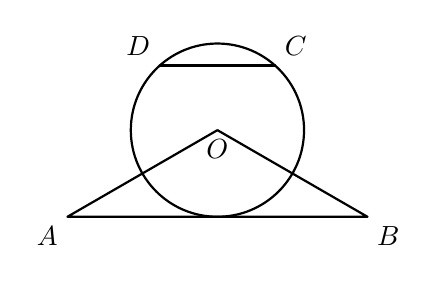
\begin{tikzpicture}[line cap=round,line join=round]
\coordinate (O) at (0,0);
\coordinate (A) at (-1.905,-1.1);
\coordinate (B) at (1.905,-1.1);
\coordinate (D) at (-0.733,0.82);
\coordinate (C) at (0.733,0.82);

\draw[thick] (O) circle (1.1);
\draw[thick] (O)--(A) (O)--(B) (A)--(B);
\draw[thick] (D)--(C);

\node[below left] at (A) {$A$};
\node[below right] at (B) {$B$};
\node[below] at (O) {$O$};
\node[above left] at (D) {$D$};
\node[above right] at (C) {$C$};
\end{tikzpicture}
\end{center}
\nopagebreak[4]
   （1）　证明：直线 \(AB\) 与 \(\odot O\) 相切；

   （2）　点 \(C,D\) 在 \(\odot O\) 上，且 \(A,B,C,D\) 四点共圆，证明：\(AB\parallel CD\)。

\end{question}
\begin{question}
\gkti{23}在直角坐标系 \(xOy\) 中，曲线 \(C_1\) 的参数方程为
\nopagebreak[4]
\[
\begin{cases}
x=a\cos t,\\
y=1+a\sin t,
\end{cases}\qquad(t\text{ 为参数},\ a>0).
\]
在以坐标原点为极点，\(x\) 轴正半轴为极轴的极坐标系中，曲线 \(C_2:\rho=4\cos\theta\)。

   （1）　说明 \(C_1\) 是哪种曲线，并将 \(C_1\) 的方程化为极坐标方程；

   （2）　直线 \(C_3\) 的极坐标方程为 \(\theta=\alpha_0\)，其中 \(\alpha_0\) 满足 \(\tan\alpha_0=2\)。若曲线 \(C_1\) 与 \(C_2\) 的公共点都在 \(C_3\) 上，求 \(a\)。

\Needspace{0.4\textheight}
\end{question}
\begin{question}
\gkti{24}已知函数 \(f(x)=|x+1|-|2x-3|\)。

   （1）　在图中画出 \(y=f(x)\) 的图象；

   （2）　求不等式 \(|f(x)|>1\) 的解集。
\nopagebreak[4]
\begin{center}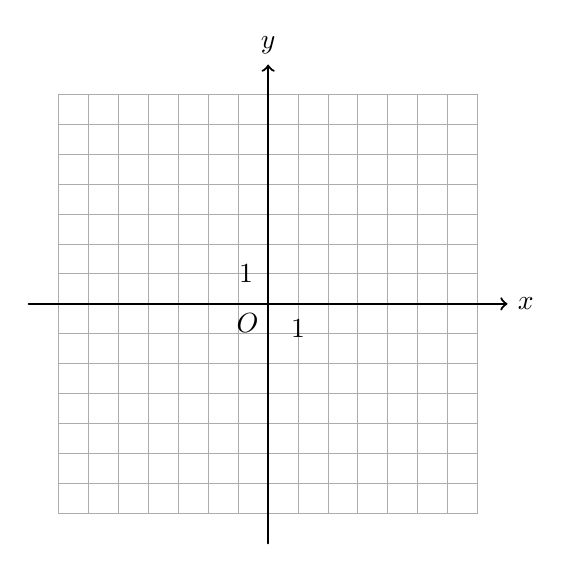
\begin{tikzpicture}[x=0.38cm,y=0.38cm,line cap=round,line join=round]
\foreach \x in {-7,-6,...,7} {
  \draw[gray!65,line width=0.35pt] (\x,-7) -- (\x,7);
}
\foreach \y in {-7,-6,...,7} {
  \draw[gray!65,line width=0.35pt] (-7,\y) -- (7,\y);
}
\draw[->,thick] (-8,0) -- (8,0) node[right] {$x$};
\draw[->,thick] (0,-8) -- (0,8) node[above] {$y$};
\node[below left] at (0,0) {$O$};
\node[left=2pt] at (0,1) {$1$};
\node[below=2pt] at (1,0) {$1$};
\end{tikzpicture}
\end{center}
\nopagebreak[4]

\end{question}